\chapter{Introduction}
\label{ch:Introduction}

Conventional energy resources such as fossil fuels and nuclear energy are not only limited supply but also pose adhere effects on the environment. Therefore, we are striving to find a cheap and renewable source of energy. Wind energy is such source of energy and is getting more popular, and have also become more affordable. Novel renewable technologies such as Vertical-Axis Wind turbines is now an interested research field.
%\index{VAWT}

\printAcron{Vertical-Axis Wind Turbine}{VAWT} are unlike the normal wind turbine. Typical wind turbines are mounted on a mast away from the ground and generates energy by spinning normal to the ground. However, a VAWT spins parallel to the ground with its hub located at the ground \cite{website:wikiVAWT}. The advantages of the vertical axis wind turbine are what makes them ideal for a source of renewable energy.  As the turbine is located at the ground, it is easily accessible and can be easily maintained. The second main advantage of the VAWT is the way it dissipates its wake. Near-wake experiments of Ferreira (2009) \cite{Ferreira}, and simulations of Vermeer (2003) \cite{Vermeer2003} have shown that the fluid past the turbine is more turbulent. Due to this higher mixing, the flow is able to smooth out much earlier. This means that it possible to places VAWTs much closer to each other and so a VAWT farm can potentially give more power per area. Furthermore, VAWTs operate independent of the flow direction, and can operate at low wind speeds (low tip-speed ratios).
%\index{HAWT}

However, with these advantages also comes some drawbacks. As the blades passes through its own wake, complex wake-body interactions take places. These have adhere effect on the blade structure and therefore is more susceptible to fatigue. This happens because the blades are constantly pitching, and complex flow behaviour such as dynamic stall and constant vortex shedding occurs \cite{SimaoFerreira2008}. This complex fluid behaviours makes it hard to predict the performance of a VAWT and this is one of the reasons why VAWTs are not mainstream. In addition, as the VAWT operates at large Reynolds number, accurate numerical methods are computationally very expensive. Therefore, it is vital to have a good understanding of the flow structure evolution and the wake generation of the VAWT using not only an efficient method, but also an accurate one.

\section{Motivation and Goal}
The goal of the research is to develop an efficient, reliable, and accurate numerical method for modelling the flow around a 2D VAWT such that one is able to deduce the correct performance characteristics of the VAWT. The two main approaches of investigate the flow is either using a numerical method to simulate the flow or by performing real-life experimental tests.

To understand the unsteady aerodynamic behaviour, \printAcron{Particle Image Velocimetry}{PIV} has been as useful tool to visualize the flow around the turbine. Ferreira et al. (2007) \cite{Ferreira2007}, have shown that it was possible to acquire flow characteristics around the blade, and these method had the accuracy to be used as validation tools. However, the downside to experimental investigation is that is it very expensive to investigate all types of configuration. Furthermore, the model sizes are limited by the dimensions of the wind tunnel and investigations with arrays of VAWT is difficult.

Numerical methods are a popular alternative as the cost of simulation and the accuracy of the models are increasing day by day. In the research field, there exists many models with various orders of accuracy. \printAcron{Actuator Disk}{AD} and \printAcron{Blade Element Momentum}{BEM} models are one of simplest models that are build upon satisfying the momentum balance of the turbine and the fluid. The advantage of theses models are that they are very quick, however they lack the accuracy that can be achieved by experimental simulation. Complex blade-wake interactions such as dynamic stalls and flow separations cannot be modeled by these methods.

	\begin{figure}[!b]
		\centering
		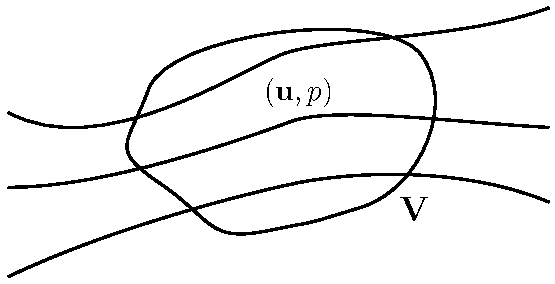
\includegraphics[width=0.4\linewidth]{figures/introduction/eulerianRF.pdf}
		\caption{Eulerian formulation of the fluid. We observe a given volume $\mathbf{V}$ and evaluate the change in properties of the fluid (from incompressible flow: velocity $\mathbf{u}$ and pressure $p$) at time passes.}
		\label{fig:eulerianRF}
	\end{figure}

To ensure more accuracy, one has to solve the Navier-Stokes equation of the flow around the turbine. \printAcron{Compuational Fluid Dynamic}{CFD} methods discretizes the fluid into smaller regions and solves the set of Navier-Stokes equation in each region (or grids). This type of formulation is known as an Eulerian method as we are evaluating the change in flow property of a given region, figure \ref{fig:eulerianRF}. In order to fully resolve the flow around the turbine, we would have to discretize the fluid at the order of the size of the vortex cores. As the vortex cores are very small (a fraction of size of the airfoil) near the blade, and very large far away from the blade (in order of size of the turbine), we must have grid size that adapts. This requires a large number of grids, as the blades are constantly  moving, and makes it computation very expensive to solve especially for arrays of turbines.

An alternative method is to use the vortex formulation of the Navier-Stokes equations, referred to as vorticity equation. This method is ideal because when describing it in Lagrangian formulation, the vorticity evolution is evaluated as interaction between vortices, and this removes the requirement of gridding, figure \ref{fig:lagrangianRF}. In addition, using simulation acceleration methods such as \printAcron{Fast Multipole Method}{FMM} and parallel computation in \printAcron{Graphical Processing Units}{GPU}, they are much more efficient that typical CFD methods and can easily be scaled to distributed computation. However, vortex method cannot inherently take in account the solid body. They require additional methods that can describe the effect of the body in the fluid and the vorticity generated from the body.

	\begin{figure}[!t]
		\centering
		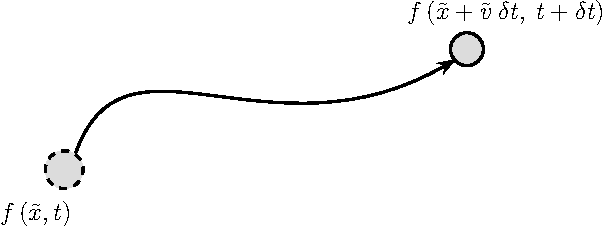
\includegraphics[width=0.4\linewidth]{figures/introduction/lagrangianRF2-crop.pdf}
		\caption{Lagrangian formulation of the fluid. We track the path of the individual fluid elements as time passes.}
		\label{fig:lagrangianRF}
	\end{figure}

So, we see that Eulerian method is accurate when describing the blade-wake interaction but are not efficient when describing multi-scale domains. Whereas, the Lagrangian method is very efficient in evolution the vorticity of the fluid, and is an ideal choice when describing the multi-scale flow characteristics. 

Therefore, in order to use the advantage of both methods, we have decided to use a domain-decomposition method, referred to as \printAcron{Hybrid Eulerian-Lagrangian Vortex Particle Method}{HVM}. In this method, the Eulerian grid method will be used at the region around the blade (near-wall region). The Lagrangian vortex method will be used in the wake region of the body. With proper coupling of these methods, we can ensure that the this numerical method can capturing not only the near-wake phenomenons such as vortex shedding, dynamic stall, and the wake-body interaction, but also the capture the large-scale flow structures such as the evolution of the VAWT wake, with efficiency and accuracy.

\section{Research Aim and Plan}

\paragraph*{Research Questions:} \textit{Is it possible to develop an efficient and accurate numerical method by an
hybrid approach where the vortex particle method is used in the wake, and the Navier-Stokes grid solver is
used at the near-body region? Will it be able to simulate real life performance characteristics of a vertical
axis wind turbine? Will it be able to predict similar performance characteristics and flow phenomena as observed from the wind tunnel experimental setup? Will it be capable of simulating the blade-wake interaction
and the dynamic stall? Where are the errors and what are their sources?}

\paragraph*{Research aim and plan:}

	\begin{itemize}
	\item Develop the Hybrid method for capturing small-scale phenomenons and large scale phenomenons.
	\item Ensure this tool is efficient, reliable, and accurate.
	\item Verify, Validate the tools with model problems.
	\item Apply the model to the 2D flow of VAWT.
	\end{itemize}

In order to answer this research questions, the goal of the project is the develop an efficient and accurate
numerical method that is not only capable of capture the small scale flow phenomena such as the dynamic stall and the vortex shedding, but is also efficient at modelling the wake evolution of VAWT. The investigation will be performed for 2D geometries and the accuracy of the model needs to established first at simpler problems before continuing to more complex problem cases.

In other words, the initial goal is to develop the hybrid vortex particle method and verify the approach. During this process, the solver will be verified and validated against test cases starting from simpler problems and gradually developing more complex features.

The final goal is to perform a simulation of a VAWT in 2D, compute its performance and validating it against experimental data. By the gradual development of the complex elements of the simulation, one can investigate the feasibility of such approach. Also, the investigation is only done for 2D currently as a full 3D simulation might be difficult and might not be feasible for the master thesis yet.

The innovativeness of this project is that such hybrid modeling has not been yet applied for the wind energy problem case. Through the parallelization of the vortex particle method in a GPU and employing solver acceleration techniques such as the FMM, this simulation could give an edge in the understanding the flow behaviour of a VAWT.

\section{Introduction to Hybrid Eulerian-Lagrangian Vortex Particle Method}

The \printAcron{Hybrid Eulerian-Lagrangian Vortex Particle Method}{HVM} is a domain-decomposition method, where the Eulerian method and the Lagrangian method solves different domains of the fluid. The domain decomposition method is simply splitting the domain of interest and using the appropriate methods in each domain. For the problem of VAWT, as the boundary is non-trivial and is the source of vorticity, the full Navier-Stokes model will be used here, and away from the body where only the convection of the vorticity field is interested, the fast and efficient vortex particle method will be used, figure \ref{fig:domainDecomposition}.

Several researches have already been done: Cottet and Koumoutsakos (2000a)\cite{Cottet2000a}, Guermond and Lu (2000) \cite{Guermond2000} simulating the advection dominated flows, Ould-Salhi et al. (2001) \cite{Ould-Salihi2001} blending finite difference and vortex method together, Winckelmans et al. (2005a) \cite{Winckelmans2005a} investigating the trailing vorticies, Daeninck (2006) \cite{Daeninck2006} implementing RANS and LES to the simulation, Stock (2010) \cite{Stock} using GPU clusters for efficiency and Speck (2011) \cite{Speck2011a} implementing researching on multipole expansion and modified interpolation kernels.

When evaluating the previous works, we see that not all domain decomposition methods are the same. The main difference differencing between the methods is their coupling strategies. Most works employ the Schwartz alternating method to couple the vortex particle method and the grid solver. The Schwartz alternating method solve the grid solver initially and couples it with the vortex method by iteratively trying to satisfy the boundary conditions. However, for this project the coupling techniques that will be used is similar to Daeninck (2006) \cite{Daeninck2006} and Stock (2010) \cite{Stock}.

	\begin{figure}[!t]
		\centering
		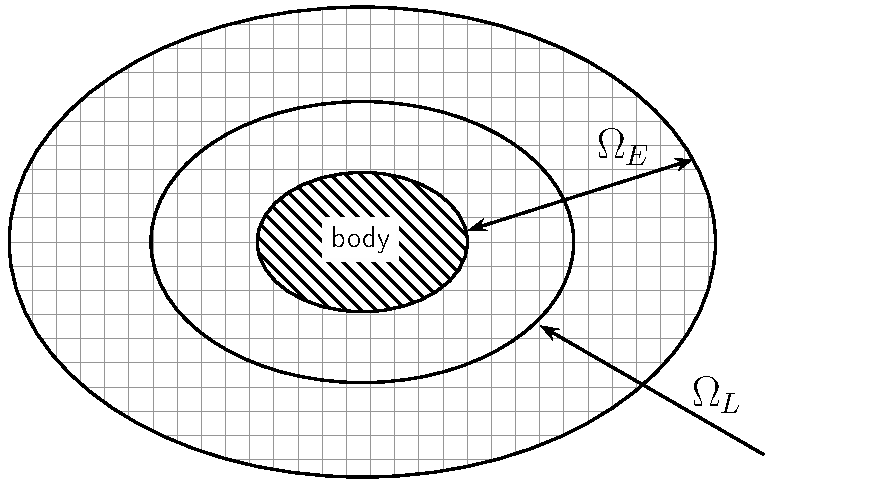
\includegraphics[width=0.5\linewidth]{figures/introduction/domainDecomposition_typical.pdf}
		\caption{Standard domain decomposition using Schwartz iteration for coupling the two methods. Eulerian domain $\Omega_E$ (near the body), and Lagrangian domain $\Omega_L$ (away from the body). Figure is based on Guermond (2000) \cite{Guermond2000}}.
		\label{fig:domainDecomposition}
	\end{figure}

\subsection{Simple coupling strategy}

	\begin{figure}[!b]
		\centering
		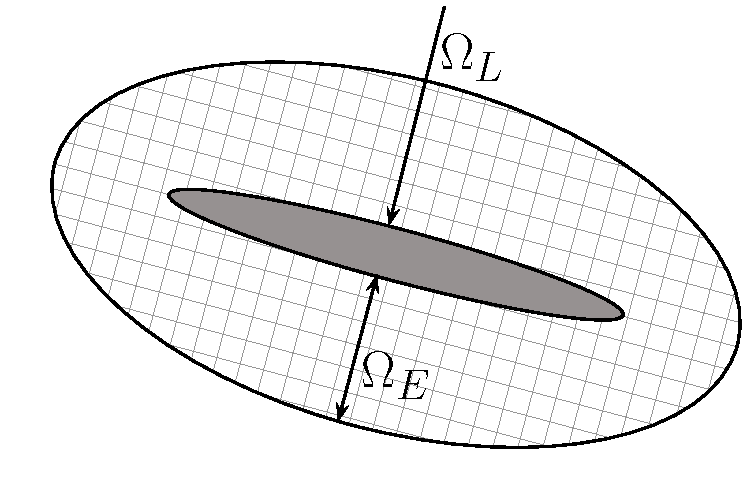
\includegraphics[width=0.5\linewidth]{figures/introduction/domainDecomposition_daenick.pdf}
		\caption{Modified domain decomposition without Schwartz alternating method. Lagrangian domain extends up to the surface of the body. Figure is based on Daeninck (2006) \cite{Daeninck2006}.}
		\label{fig:domainDecomposition_daenick}
	\end{figure}

This new approach is much simpler and only a single iteration is needed for the coupling. The basic procedure is to solve the vortex method in the whole domain using relatively coarse evaluation, then use the grid solver in the near wall region to capture the detailed features of the boundary layer and transfer the vorticity field at this region to the vortex particles, figure \ref{fig:domainDecomposition_daenick}. The functionality of this strategy has been demonstrated by Daeninck and was found to be significantly faster than the Schwartz coupling strategy.

The \underline{features of the simple coupling strategy} can summarized as follows:

	\begin{itemize}
	\item Eulerian method is used to resolve the near-wall region, referred to as Eulerian domain $\Omega_E$. With this implementation, subtle features of the boundary layer (such as flow separation) can be resolved with great accuracy.
	\item Lagrangian method is used to capture the wake, referred to as Lagrangian domain $\Omega_L$. Lagrangian method is used to efficiently evolve the wake.
	\item The accurate solution of the Eulerian domain is transfered to the Lagrangian domain according to the coupling strategies of Daeninck \cite{Daeninck2006} and Stock \cite{Stock}.
	\item The boundary conditions for the Eulerian domain is retrieved from the Lagrangian domain.
	\end{itemize}


	\begin{figure}[!b]
		\centering
		\begin{tikzpicture}
			[node distance=.8cm, start chain=going below,]
			\node[punktchain, join] (correct) {Correct the Lagrangian domain};
		    \node[punktchain, join] (evolveL) {Evolve the Lagrangian solution};
		    \node[punktchain, join] (bcE)     {Determine the Eulerian boundary conditions};
		    \node[punktchain, join] (evolveE) {Evolve the Eulerian solution};
		\end{tikzpicture}
		\caption{Flowchart of the simple coupling strategy. The flowchart shows the procedure to evolve both methods from $t_n$ to $t_{n+1}$.}
		\label{fig:flowchart_simpleCoupling}
	\end{figure}

Figure \ref{fig:flowchart_simpleCoupling} shows the overview to the simple coupling strategy. The detailed algorithm to the simple coupling strategy follows from Daeninck \cite{Daeninck2006}.

The \underline{simple coupling algorithm} can be summarized as follows:

	\begin{enumerate}
	\item \textbf{Correct Lagrangian:} Use the solution of the Eulerian domain $\Omega_E$ (in the near-wall region) to correct the solution of the Lagrangian domain $\Omega_L$ overlapping in the Eulerian domain.  
	\item \textbf{Evolve Lagrangian:} With the modified solution, evolve the Lagrangian solution from $t_n$ to $t_{n+1}$.
	\item \textbf{Determine Eulerian boundary conditions:} Use the Lagrangian solution of $t_n$ and $t_{n+1}$ to determine the boundary conditions of the Eulerian domain.
	\item \textbf{Evolve Eulerian:} With the boundary condition, evolve the Eulerian solution from $t_n$ to $t_{n+1}$.
	\end{enumerate}
	
This is the basic approach for coupling the Eulerian method in the Eulerian domain $\Omega_E$ with the Lagrangian method in the Lagrangian domain $\Omega_L$ without the iterative Schwartz algorithm. In addition, the second difference between the classical hybrid method is that the Lagrangian method handles the boundary conditions differently. Typically during the evolution process of the Lagrangian domain, vorticity is shed from body. However, in this coupling strategy, the Lagrangian method under-resolves the boundary and cannot be used to resolve the vorticity flux. Instead, we use the Eulerian method to resolve the boundary and interpolate the newly generated vorticity into the Lagrangian domain.

However, there as some \underline{assumptions} that we must satisfy, for this coupling strategy to be valid:

	\begin{enumerate}
	\item At $t_n$, before the evolution of both method to $t_{n+1}$, the Lagrangian solution matches Eulerian solution at the near-wall region.
	\item After the evolution to $t_{n+1}$, the deviation of the Lagrangian solution (due to lack of vorticity flux at Lagrangian boundary), is minimal.
	\item Even though the Lagrangian domain is under-resolved in the near-wall region, it should be able to provide accurate boundary conditions for the Eulerian external boundary.
	\end{enumerate}


\section{Verification and Validation Test Cases}

The test-cases that are used for this thesis are summarized as given:

	\begin{description}
	\item[Lamb-Oseen vortex] \cite{Lamb1993} \cite{Tryggeson2007} \hfill\\
	Lamb-Oseen vortex test case is an analytical solution derived from the diffusion equation, and is a test case for unbounded flow (without any wall). This is the first model that will be used to validate the Lagrangian method and Eulerian method separately. This test case focuses on the diffusion of the vortcity is an ideal to verify and validate the convection and diffusion of the vorticity.
	\item[Clercx-Bruneau dipole] \cite{Clercx2006}\hfill\\
	The Clercx-Bruneau dipole test case is the simple case of dipole colliding with a wall and is used to verify the coupling of the methods. This test cases focuses on the generation of vorticity from the wall and is ideal to verify and validate the coupling.
	\item[Impulsively started cylinder] \cite{LEONARD1995} \cite{Chang2006} \cite{Chassaing1986} \cite{Lecointe1985}\hfill\\
	The impulsively started cylinder test case focuses on the forces acting on the cylinder. This test case is used to verify and validate the lift and drag evolution of the cylinder exposed to free-stream flow.
	\item[Elliptic Airfoil] \cite{Nair1997}\hfill\\
	The elliptic airfoil test cases focuses on the flow separation past a lifting body. The elliptic airfoil is pitched at high angle of attack and the flow past the airfoil is comparatively unsteady and undergoes phenomenons such as laminar separation bubble, flow separation and karman vortex shedding from the trailing edge of the airfoil. This helps us ensure coupling process is sound for complex flow phenomenons.
	\end{description}

%\todo{add picture here}
\section{Methodology}
The initial steps of the development of the hybrid vortex methods is as follows:

	\begin{itemize}
	\item Develop the vortex particle method
	\item Validate the vortex particle method against a Lamb-Oseen convection test case.
	\item Develop the vortex panel method to deal with the boundaries for the vortex particle calculation. 
	\item Validate the vortex panel method by solving a potential flow around a cylinder.
	\item Develop the grid solver that is based on the Finite Element method. 
	\item Validate the grid solver against test cases: impulsively starting cylinder, dipole-Wall interaction.
	\end{itemize}

Once all the components have been validated, the methods will be coupled and validated against similar test cases.

	\begin{itemize}
	\item Couple vortex particle, vortex panel and grid solver together.
	\item Validate it with the previous generated test case solution.
	\item Introduce more complicated phenomenons: multiple geometry (i.e multiple grid meshes) and moving boundaries, if it feasible in the constraints of a master thesis.
	\end{itemize}

If the coupled solver has been validated with the test cases, the final step will be to simulated the flow around a VAWT and investigating the performance vs. numerical and experimental data.

%\subsection{Project Plan}

\section{Thesis Outline}

\todo{Update this section}

%\section{Research question}
%\label{sec:ResearchQuestion}
%
%\section{Research objective}
%\label{sec:ResearchObjective}
%
%\section{Importance of study}
%
%\section{Scope of thesis}
%\label{sec:scope}
%
%\section{Structure of the report}
%\label{sec:Structure of the report}

